%\documentclass[varwidth=true, border=5pt, convert={size=640x}]{standalone}
\documentclass{beamer}
\usepackage[scale=1.25,size=custom,width=84.1,height=118.9,orientation=portrait]{beamerposter}
\geometry{margin=10mm}
\usepackage{tikz}
\usetikzlibrary{positioning,shapes,arrows,backgrounds,calc,fit,trees,arrows.meta,external}
\newlength{\myimscale}

\usepackage[export]{adjustbox}
\usepackage{multirow}

\tikzstyle{dummy} = []
\tikzstyle{line} = [draw, line width=1pt, -latex']
\tikzstyle{headless_line} = [draw, line width=1pt, -]
\tikzstyle{default}    = [rectangle, text centered, rounded corners, text=black, font=\sffamily\footnotesize, align=center]
\tikzstyle{default_text}    = [rectangle, text width=18cm, text=black,anchor=north west, font=\sffamily]
\tikzstyle{boxwhite} = [default, fill=white, rounded corners=0.2cm]
\tikzstyle{cp}    = [default, fill=seaborn_blue, text=white, text width=4.5cm, minimum height=1.0cm]
\tikzstyle{pw}    = [cp, fill=seaborn_green]
\tikzstyle{kcw}    = [cp, fill=seaborn_orange]
\tikzstyle{wannier90}    = [cp, fill=seaborn_cyan]
\tikzstyle{bespoke}    = [cp, fill=seaborn_magenta]
\tikzstyle{observable}    = [cp, fill=seaborn_red]
\tikzset{
  -|-/.style={
    to path={
      (\tikztostart) -| ($(\tikztostart)!#1!(\tikztotarget)$) |- (\tikztotarget)
      \tikztonodes
    }
  },
  -|-/.default=0.5,
  |-|/.style={
    to path={
      (\tikztostart) |- ($(\tikztostart)!#1!(\tikztotarget)$) -| (\tikztotarget)
      \tikztonodes
    }
  },
  |-|/.default=0.5,
}

\newlength{\myyshift}
\setlength{\myyshift}{0.1cm}

\newcommand{\bra}[1]{\langle #1|}
\newcommand{\braket}[2]{\langle #1|#2\rangle}
\newcommand{\braopket}[3]{\langle #1|#2|#3\rangle}
\newcommand{\ket}[1]{|#1\rangle}
\newcommand{\nline}{\nonumber \\}
\newcommand{\Trace}{\mathrm{Tr}}

\usepackage{sansmath}
\sansmath
\usepackage{helvet}
\setbeamerfont{normal text}{family=helvet}
\setbeamerfont{local structure}{family=helvet}
\setbeamerfont*{block title}{series=\bf}
\definecolor{kgrey}{HTML}{2b2828}
\definecolor{kgrey_light}{HTML}{d2cfcf}
\definecolor{kgrey_verylight}{HTML}{eeeded}
\definecolor{marvel_red}{HTML}{d73530}
\setbeamercolor{block body alert}{fg=white, bg=kgrey}
\setbeamercolor{block title}{bg=kgrey, fg=white}
\setbeamercolor{block body}{fg=kgrey, bg=white}
\setbeamertemplate{itemize item}{\color{kgrey}$\blacktriangleright$}
\beamertemplatenavigationsymbolsempty

% Definitions of colours used in seaborn for use in latex
\definecolor{seaborn_bg_grey}{HTML}{eaeaf2}
% \definecolor{seaborn_bg_grey}{HTML}{a3a3a9}
\definecolor{seaborn_bg_grey_dark}{HTML}{d2d2d9}
\definecolor{seaborn_bg_grey_darker}{HTML}{a3a3a9}
\definecolor{seaborn_bg_grey_half}{HTML}{f4f4f8}

\definecolor{seaborn_blue}{HTML}{4c72b0}
\definecolor{seaborn_orange}{HTML}{da8558}
\definecolor{seaborn_green}{HTML}{55a868}
\definecolor{seaborn_red}{HTML}{c44e52}
\definecolor{seaborn_magenta}{HTML}{8172b2}
\definecolor{seaborn_yellow}{HTML}{ccb974}
\definecolor{seaborn_cyan}{HTML}{64b5cd}

\definecolor{seaborn_muted_blue}{HTML}{4878cf}
\definecolor{seaborn_muted_green}{HTML}{6acc65}
\definecolor{seaborn_muted_red}{HTML}{d65f5f}
\definecolor{seaborn_muted_magenta}{HTML}{b47cc7}
\definecolor{seaborn_muted_yellow}{HTML}{c4ad66}
\definecolor{seaborn_muted_cyan}{HTML}{77bedb}

\definecolor{seaborn_pastel_blue}{HTML}{92c6ff}
\definecolor{seaborn_pastel_green}{HTML}{97f0aa}
\definecolor{seaborn_pastel_red}{HTML}{ff9f9a}
\definecolor{seaborn_pastel_magenta}{HTML}{d0bbff}
\definecolor{seaborn_pastel_yellow}{HTML}{fffea3}
\definecolor{seaborn_pastel_cyan}{HTML}{b0e0e6}

\definecolor{seaborn_bright_blue}{HTML}{003fff}
\definecolor{seaborn_bright_green}{HTML}{03ed3a}
\definecolor{seaborn_bright_red}{HTML}{e8000b}
\definecolor{seaborn_bright_magenta}{HTML}{8a2be2}
\definecolor{seaborn_bright_yellow}{HTML}{ffc400}
\definecolor{seaborn_bright_cyan}{HTML}{00d7ff}

\definecolor{seaborn_dark_blue}{HTML}{001c7f}
\definecolor{seaborn_dark_green}{HTML}{017517}
\definecolor{seaborn_dark_red}{HTML}{8c0900}
\definecolor{seaborn_dark_magenta}{HTML}{7600a1}
\definecolor{seaborn_dark_yellow}{HTML}{b8860b}
\definecolor{seaborn_dark_cyan}{HTML}{006374}

\definecolor{seaborn_colorblind_blue}{HTML}{0072b2}
\definecolor{seaborn_colorblind_green}{HTML}{009e73}
\definecolor{seaborn_colorblind_red}{HTML}{d55e00}
\definecolor{seaborn_colorblind_magenta}{HTML}{cc79a7}
\definecolor{seaborn_colorblind_yellow}{HTML}{f0e442}
\definecolor{seaborn_colorblind_cyan}{HTML}{56b4e9}


\usepackage{siunitx,booktabs}
\renewcommand{\ttdefault}{pcr}

\usepackage{minted}
\usemintedstyle{friendly}
% \usemintedstyle{gruvbox}
% \definecolor{gruvbox_dark_bg}{HTML}{282828}
% \definecolor{gruvbox_fg}{HTML}{ebdbb2}
% \setminted[python]{bgcolor=gruvbox_dark_bg}
% \setminted[json]{bgcolor=gruvbox_dark_bg}
% \setminted[shell-session]{style=gruvbox_plain, bgcolor=gruvbox_dark_bg}


\usepackage[backend=biber, bibencoding=utf8, style=science, maxbibnames=1, maxcitenames=1, 
            sorting=none, giveninits=true, isbn=false, doi=false, url=false]{biblatex}
% Bibliography %%%%%%%%%%%%%%%%%%%%%%%%%%%%%%%%%%%%%%%%%%%%%%%%%%%%%%%%%%%%%%%%%%%%%%%%%%%%%%%%%%%%%
% Note that different styles might not turn [7,3,4,5] into [3-5,7]. Be careful!
\renewbibmacro{in:}{}                           % Remove the "In:"
\DeclareFieldFormat{pages}{\mkfirstpage{#1}} % Only have first page appear
% % Remove the period between volume and number
% \renewbibmacro{volume+number+eid}{%
%     \printfield{volume}%
%     \setunit{\addcomma\space}%
%     \printfield{number}}
\AtEveryBibitem{%
  \clearfield{shorttitle}%
  \clearfield{month}%
  \clearfield{abstract}%
  \clearfield{title}%
  % \ifentrytype{article}{%
  %    \clearfield{title}%
  % }{}
}
% \newcommand{\onlinecite}[1]{\hspace{-1 ex} \nocite{#1}\citenum{#1}} 

% Make all authors be listed as F. M. Surname (in conjunction with giveninits=true)
\DeclareNameAlias{default}{first-last}


% An inline citation without square brackets
% (From https://tex.stackexchange.com/questions/25962/biblatex-cite-command-to-create-numeric-citation-without-parentheses)
% A simple modification of code from /usr/local/texlive/2016/texmf-dist/tex/latex/biblatex/cbx/numeric-comp.cbx
\DeclareCiteCommand{\onlinecite}%[\mkbibbrackets]
{\usebibmacro{cite:init}%
  \usebibmacro{prenote}}
{\usebibmacro{citeindex}%
  \usebibmacro{cite:comp}}
{}
{\usebibmacro{cite:dump}%
  \usebibmacro{postnote}}



% Make title of citations a hyperlink
% (From https://tex.stackexchange.com/questions/48400/biblatex-make-title-hyperlink-to-dois-url-or-isbn)
\newbibmacro{string+doiurl}[1]{%
  \iffieldundef{doi}{%
    \iffieldundef{url}{%
      \textit{#1}%
    }{%
      \href{\thefield{url}}{\textit{#1}}%
    }%
  }{%
    \href{http://dx.doi.org/\thefield{doi}}{\textit{#1}}%
  }%
}

\DeclareFieldFormat{howpublished}{\texttt{\url{#1}}}
% \DeclareFieldFormat{title}{\usebibmacro{string+doiurl}{\mkbibemph{#1}}}
\DeclareFieldFormat{title}{\usebibmacro{string+doiurl}{#1}}
\DeclareFieldFormat[article,incollection]{title}%
{\usebibmacro{string+doiurl}{#1}}
\DeclareFieldFormat{journaltitle}{\textsf{#1}}

% Ensuring \citeauthor is a hyperlink to the bib entry
\DeclareCiteCommand{\citeauthor}
{\boolfalse{citetracker}%
  \boolfalse{pagetracker}%
  \usebibmacro{prenote}}
{\ifciteindex
  {\indexnames{labelname}}
  {}%
  \printtext[bibhyperref]{\printnames{labelname}}}
{\multicitedelim}
{\usebibmacro{postnote}}

% Ensuring tildes in urls survive
\DeclareSourcemap{
  \maps{
    \map{
      \step[fieldsource=howpublished,
        match=\regexp{\$\\sim\$},
        replace=\regexp{\~}]
    }
    \map{
      \step[fieldsource=url,
        match=\regexp{\$\\sim\$},
        replace=\regexp{\~}]
    }
  }
}

\DeclareSourcemap{
  \maps[datatype=bibtex,overwrite=False]{
   \map{
     \step[fieldsource=journal,
           match={Journal of Chemical Theory and Computation},
           replace={JCTC}]
     \step[fieldsource=journal,
           match={Reviews of Modern Physics},
           replace={Rev. Mod. Phys.}]
     \step[fieldsource=journal,
           match={Reports on Progress in Physics},
           replace={Rep. Prog. Phys.}]
     \step[fieldsource=journal,
           match={Physical Review Letters},
           replace={Phys. Rev. Lett.}]
     \step[fieldsource=journal,
           match={Physical Review},
           replace={Phys. Rev.}]
     \step[fieldsource=journal,
           match={B - Condensed Matter and Materials Physics},
           replace={B}]
     \step[fieldsource=journal,
           match={Journal of Chemical Physics},
           replace={J. Chem. Phys.}]
     \step[fieldsource=journal,
           match={Annual Review of Materials Research},
           replace={Annu. Rev. Mater. Res.}]
   }
  }
}

\addbibresource{/home/elinscott/code/koopmans/src/koopmans/references.bib}
\setbeamercolor*{bibliography entry author}{fg=kgrey}
\setbeamercolor*{bibliography entry title}{fg=kgrey}
\setbeamercolor*{bibliography entry note}{fg=kgrey}
\setbeamertemplate{bibliography item}{}

\usepackage{anyfontsize}

\usepackage{tcolorbox}
\tcbuselibrary{skins,hooks}
\tcbset{colframe=structure,fonttitle=\bfseries,beamer, clip upper, boxsep=0pt, sharp corners=all, no shadow, left skip=0pt, right skip=0pt, coltext=white}

\begin{document}
\newcommand{\citeauthoryear}[1]{\citeauthor{#1} \citeyear{#1}}
\begin{frame}[t]{}

    \vspace{-0.001\paperheight}
    \begin{beamercolorbox}[wd=\textwidth,sep=1em]{}
        \begin{minipage}[height=0.15\textwidth]{0.15\textwidth}
            
\includegraphics[width=\textwidth]{figures/marvel_trimmed.png}
        \end{minipage}
        \hfill
        \setbeamercolor{marvelheader}{fg=white,bg=marvel_red}
        \begin{minipage}[height=0.15\textwidth]{0.4\textwidth}
        \begin{beamercolorbox}[wd=\textwidth,sep=1em]{marvelheader}
            \centering
            \bf
            {\fontsize{100}{120}\selectfont Pillar 4}
        \end{beamercolorbox}
        \end{minipage}
        \hfill
        \begin{minipage}[height=0.15\textwidth]{0.15\textwidth}
        
\includegraphics[width=\textwidth]{/home/elinscott/Pictures/epfl_logos/red_cropped.eps}
        \end{minipage}
    \end{beamercolorbox}
    \setbeamercolor{banner}{fg=kgrey,bg=white}
    \begin{beamercolorbox}[wd=\textwidth,sep=1em]{banner}
        \bf
        \begin{center}
            {
\includegraphics[width=0.55\paperwidth]{figures/koopmans_grey_on_transparent.png}}

            % \vspace{-11em}
            % \hbox{\hspace{0.77\textwidth}
            %     \begin{tcolorbox}[enhanced jigsaw, width=16cm, opacityback=0, colframe=seaborn_red, coltext=seaborn_red, left=10pt, bottom=10pt, top=10pt, right=10pt, tikz={rotate=30,transform shape}, boxrule=5mm]
            %         \begin{center}
            %             % \includegraphics[height=1cm]{./figures/qe_logo_high_res_cropped.jpg}
            %             % \bf \huge\ \raisebox{0.3cm}{+}\,
            %             % \includegraphics[height=1cm]{./figures/python_logo.png}

            %             \bf \Huge OUT NOW!
            %         \end{center}
            %     \end{tcolorbox}
            % }

            \vspace{-1em}
            \LARGE
            \emph{an open-source package for accurately and efficiently predicting spectral properties with Koopmans functionals}

            \vspace{1em}
            \large
            Edward Linscott,\textsuperscript{1} Nicola Colonna,\textsuperscript{2,3} Riccardo De Gennaro,\textsuperscript{1} and Nicola Marzari\textsuperscript{1,2,4}
            \vspace{1em}
        \end{center}
    \end{beamercolorbox}

    \vspace{-0.001\paperheight}
    \setbeamercolor{background}{fg=white,bg=seaborn_bg_grey}
    \begin{beamercolorbox}[ht=0.675\paperheight,wd=\textwidth]{background}

        \begin{columns}[t]
            \begin{column}{0.37\linewidth}
                \begin{block}{Summary}
                    \texttt{koopmans} contains everything you need to run a Koopmans functional calculation without expert knowledge, including implementations of Koopmans functionals in \textsc{Quantum ESPRESSO} as well as automated workflows.
                \end{block}

                \vspace{1.8ex}

                \begin{block}{1. What are Koopmans functionals?}
                    \nocite{Dabo2009,Dabo2010,Borghi2014,Colonna2018,Nguyen2018,Colonna2019,DeGennaro2022,Colonna2022,Linscott2023}
                    Koopmans functionals are a class of functionals that aim to reproduce spectral properties (charged excitations) and total energies on the same footing, enforcing a generalised piecewise linearity condition:
                    \vspace{0.125em}
                    \begin{equation*}
                        E_\mathrm{Koopmans} = E_\mathrm{DFT} + \sum_i \alpha_i \biggl[ \underbrace{- \left(E_\mathrm{DFT} - \left.E_\mathrm{DFT}\right|_{{f_i}=0}\right)}_{\substack{\text{removes the erroneous} \\ \text{curvature}}} \underbrace{+ f_i \eta_i}_{\substack{\text{restores the}\\ \text{correct linearity}}} \biggr]
                    \end{equation*}

                    \vspace{1.35em}
                \end{block}

            \end{column}

            \begin{column}{0.57\linewidth}

                \begin{block}{2. Workflows}
                    \vspace{0.5ex}
                    \begin{center}
                        \begin{minipage}{\linewidth}
                            Supercell implementation

                            \vspace{-2ex}
                            \begin{tikzpicture}[font=\tiny, x=6.5cm, y=2cm]
   \begin{scope}[scale=0.7, every node/.style={scale=0.7}]
   \begin{pgfonlayer}{background}
      % \node[fit= (KC init) (empty label) (filled label) (sc loop 1) (converged label), fill=seaborn_bg_grey, inner sep=0.5cm] (calculating screening) {};
      % \node [dummy, above=0cm of calculating screening, font=\sffamily]{Calculating screening parameters};
      \fill [seaborn_bg_grey] (-2.1,-0.8) rectangle (1.3,4.6);
      \node at (-2.1, 4.6) [default_text, font=\footnotesize] {Initialisation (molecules)};
      \fill [seaborn_bg_grey] (-2.1,-4.6) rectangle (1.3,-1.2);
      \node at (-2.1, -1.2) [default_text, font=\footnotesize] {Initialisation (solids)};
      \fill [seaborn_bg_grey] (1.4,-4.6) rectangle (6.9,4.6);
      \node at (1.4, 4.6) [default_text, font=\footnotesize, text width=4.5cm] {Calculating screening parameters};
      \fill [seaborn_bg_grey] (7,-4.6) rectangle (8,4.6);
      \node at (7, 4.6) [default_text, font=\footnotesize, text width=6cm] {Final calculation};
      \fill [seaborn_bg_grey] (8.1,-4.6) rectangle (9.1,4.6);
      \node at (8.1, 4.6) [default_text, font=\footnotesize, text width=6cm] {Postprocessing (solids)};
   \end{pgfonlayer}

   % Key
   \node at (5.84, 5.25) [cp, text width=2.4cm, minimum height=1.7cm, font=\tiny] {\texttt{kcp}};
   \node at (6.44, 5.25) [kcw, text width=2.4cm, minimum height=1.7cm, font=\tiny] {\texttt{kcw}};
   \node at (7.04, 5.25) [pw, text width=2.4cm, minimum height=1.7cm, font=\tiny] {\texttt{pw}};
   \node at (7.64, 5.25) [wannier90, text width=2.4cm, minimum height=1.7cm, font=\tiny] {\texttt{wannier}};
   \node at (8.24, 5.25) [bespoke, text width=2.4cm, minimum height=1.7cm, font=\tiny] {bespoke code};
   \node at (8.84, 5.25) [observable, text width=2.4cm, minimum height=1.7cm, font=\tiny] {quantity of interest};

   % Initialisation
   % Option 1
   \node at (-1, 2.9) [cp] (DFT init) {DFT};
   \node at (0, 2.9) [cp] (PZ innerloop) {PZ unitary rotation};
   \path [line] (DFT init) -- (PZ innerloop);

   % OR
   \node at (-0.5, 1.9) [default] (or) {or};

   % Option 2
   \node at (-0.5, 0.9) [cp] (PZ init) {PZ};

   % Solids
   \node at (-1.5, -2.9) [pw] (pw DFT init) {DFT (primitive cell)};
   \node at (-0.5, -2.9) [wannier90] (wannierize) {wannierize};
   \node at (0.5, -2.9) [bespoke] (unfold) {fold to supercell};
   \path [line] (pw DFT init) -- (wannierize);
   \path [line] (wannierize) -- (unfold);

   % Calculating screening parameters
   \node at (2, 0) [cp] (KC init) {$\alpha_0$KI/$\alpha_0$KIPZ};

   \path let
   \p1 = (PZ innerloop),
   \p2 = (unfold.east)
   in
   coordinate (dummy) at (\x2, \y1);
   \path let
   \p1 = (PZ init),
   \p2 = (unfold.east)
   in
   coordinate (dummy2) at (\x2, \y1);
   \path [line] (PZ innerloop) -- (dummy) to[-|-=0.3] ([yshift=2\myyshift]KC init.west);
   \path [line] (PZ init.east) -- ([xshift=-3.5\myyshift]dummy2) to[-|-=0.3] (KC init.west);
   \path [line] ([yshift=-2\myyshift]unfold.east) to[-|-=0.3] ([yshift=-2\myyshift]KC init.west);

   % KI filled %%%%%%%%%%%%%%%%%%%%%%%%%%%%%%%%%%%%%%%%%%%%%%%%%%

   % calculations
   \node at (3, 3) [cp] (N-1_filled) {DFT/$\alpha_0$KIPZ ($N-1$)};
   \node at (3, -3) [cp] (N+1_empty) {DFT/$\alpha_0$KIPZ ($N+1$)};

   \path [line] (KC init) to[-|-] (N-1_filled);
   \path [line] (KC init) to[-|-] (N+1_empty);

   % results
   \node at (4, 3) [observable] (EN-1_filled) {$E_i(N-1)$};
   \node at (4, 2) [observable] (lambda0_filled) {$\lambda^{0}_{ii}(1)$};
   \node at (4, 1) [observable] (lambda_filled) {$\lambda^{\alpha_0}_{ii}(1)$};
   \node at (4, 0) [observable] (EN) {$E(N)$};
   \node at (4, -1) [observable] (lambda_empty) {$\lambda^{\alpha_0}_{ii}(0)$};
   \node at (4, -2) [observable] (lambda0_empty) {$\lambda^{0}_{ii}(0)$};
   \node at (4, -3) [observable] (EN+1_empty) {$E_i(N+1)$};

   \path [line] (KC init) -- (EN);
   \path [line] (KC init.east) to[-|-] (lambda_filled.west);
   \path [line] (KC init.east) to[-|-] (lambda_empty.west);

   \path [line] (KC init) to[-|-] (lambda0_filled);
   \path [line] (KC init) to[-|-] (lambda0_empty);
   \path [line] (N-1_filled) -- (EN-1_filled);
   \path [line] (N+1_empty) -- (EN+1_empty);

   % alpha parameters
   \node at (5, 1.5) [observable] (alpha filled) {$\alpha_{i \in \text{filled}}$};
   \node at (5, -1.5) [observable] (alpha empty) {$\alpha_{i \in \text{empty}}$};

   \path [line] (lambda_filled) to[-|-] (alpha filled);
   \path [line] ([yshift=\myyshift]EN.east) to[-|-] (alpha filled.west);
   \path [line] (lambda0_filled) to[-|-] (alpha filled);
   \path [line] (EN-1_filled) to[-|-] (alpha filled);

   \path [line] (lambda_empty) to[-|-] (alpha empty);
   \path [line] ([yshift=-\myyshift]EN.east) to[-|-] (alpha empty.west);
   \path [line] (lambda0_empty) to[-|-] (alpha empty);
   \path [line] (EN+1_empty) to[-|-] (alpha empty);

   % SC check
   \coordinate (sc check) at (6, 0);
   \path [headless_line] (alpha empty) to[-|-] (sc check);
   \path [headless_line] (alpha filled) to[-|-] (sc check);

   % Final calc
   \node at (7.5, 0) [cp] (final KI) {$\alpha$KI/$\alpha$KIPZ};
   \path [line] (sc check) -- node [midway, above, font=\sffamily\tiny] (converged label) {$\{\alpha_i\}$ converged} (final KI);

   % Postproc
   \node at (8.6, 0) [bespoke] (upfold) {unfold to primitive cell};
   \path [line] (final KI) -- (upfold);
\end{scope}

   % Boxes
   % Screening parametere
   \node [boxwhite, fit= (N-1_filled) (EN-1_filled),
      draw, dashed, fill opacity=0, inner sep=0.15cm](filled box){};
   \node [dummy, above=-0.2cm of filled box, font=\sffamily](filled label){\tiny one per unique filled orbital (index $i$)};
   \node [boxwhite, fit= (N+1_empty) (EN+1_empty),
      draw, dashed, fill opacity=0, inner sep=0.15cm](empty box){};
   \node [dummy, below=-0.2cm of empty box, font=\sffamily](empty label){\tiny one per unique empty orbital (index $i$)};

   % SC loop
   \node [below=-0.4cm of empty label] (sc loop y) {};
   \path let
   \p1 = (sc check),
   \p2 = (sc loop y)
   in
   coordinate (sc loop 1) at (\x1, \y2);
   \path [line] (sc check) -- node [midway, right, font=\sffamily\tiny, align=left] (not converged label) {$\{\alpha_i\}$ not\\converged} (sc loop 1) -| (KC init.south);


   % \onslide<2->{
   %    \node at (3.5, 0) [default_text, fill=white, opacity=0.9, text opacity=1, anchor=center, minimum height=5cm, text width=7.5cm, execute at begin node=\setlength{\baselineskip}{30pt}] (nc text) {
   %       \huge Riccardo De Gennaro
   %       \textbf{M22.00004} / paper in preparation
   %    };
   %    \node[right = -0.2cm of nc text, anchor=west]{\includegraphics[height=5cm]{figures/riccardo_degennaro.jpg}};
   % }

\end{tikzpicture}


                            \vspace{-2ex}
                            \noindent Primitive cell implementation

                            \vspace{0.5ex}
                            \begin{tikzpicture}[font=\tiny, x=6.5cm, y=2cm, scale=0.7, every node/.style={scale=0.7}]
   \begin{pgfonlayer}{background}
      \fill [seaborn_bg_grey] (-2.2,-1) rectangle (1.2,1.5);
      \node at (-2.2, 1.5) [default_text] {\footnotesize Initialisation};
      \fill [seaborn_bg_grey] (1.3,-1) rectangle (3.7,1.5);
      \node at (1.3, 1.5) [default_text] {\footnotesize Calculating screening parameters};
      \fill [seaborn_bg_grey] (3.8,-1) rectangle (5.2,1.5);
      \node at (3.8, 1.5) [default_text, text width=7cm] {\footnotesize Final calculation};
      % \fill [seaborn_bg_grey] (8.1,-1) rectangle (9.1,1.5);
      % \node at (8.1, 1.5) [default_text, text width=3.5cm] {\large Postprocessing};
   \end{pgfonlayer}

   % % Key
   % \node at (3.45, 2.15) [pw, text width=1.4cm, minimum height=0.7cm] {\texttt{pw}};
   % \node at (3.95, 2.15) [wannier90, text width=1.4cm, minimum height=0.7cm] {\texttt{wannier90}};
   % \node at (4.45, 2.15) [bespoke, text width=1.4cm, minimum height=0.7cm, font=\tiny] {bespoke code};
   % \node at (4.95, 2.15) [observable, text width=1.4cm, minimum height=0.7cm, font=\tiny] {quantity of interest};

   % Initialisation
   % Solids
   \node at (-1.5, 0) [pw] (pw DFT init) {DFT};
   \node at (-0.5, 0) [wannier90] (wannierize) {wannierize};
   \node at (0.5, 0) [observable] (unfold) {$\{\ket{w_i}\}$};
   \path [line] (pw DFT init) -- (wannierize);
   \path [line] (wannierize) -- (unfold);

   % Calculating screening parameters
   \node at (2, 0) [kcw] (KC screen) {DFPT calculation};
   \node at (3, 0) [observable] (alphas) {$\{\alpha_i\}$};
   \path [line] (unfold) -- (KC screen);
   \path [line] (KC screen) -- (alphas);

   % Final calc
   \node at (4.5, 0) [kcw] (KC ham) {$\alpha_0$KI/$\alpha_0$KIPZ};
   \path [line] (alphas) -- (KC ham);

   % \onslide<4->{
   %    \node at (1, 0) [default_text, fill=white, opacity=0.9, text opacity=1, anchor=center, minimum height=5cm, text width=7cm, execute at begin node=\setlength{\baselineskip}{30pt}] (nc text) {
   %       \huge Nicola Colonna
   %       \textbf{A20.00002} /
   %       paper in preparation
   %    };
   %    \node[right = -0.2cm of nc text, anchor=west]{\includegraphics[height=5cm]{figures/nicola_colonna.png}};
   % }

\end{tikzpicture}

                        \end{minipage}
                    \end{center}
                \end{block}
            \end{column}

        \end{columns}

        \vspace{1em}
        \begin{columns}
            \begin{column}{0.968\textwidth}
                \begin{block}{3. Example results}
                    \setlength{\tabcolsep}{5pt}
                    \renewcommand{\arraystretch}{1}
                    \vspace{0.7em}
                    \hbox{

                        \begin{minipage}[0.25\textwidth]{0.4\textwidth}

                            \textbf{Koopmans functionals give band structures and orbital energies as accurate as state-of-the-art GW, at a fraction of the computational cost.}

                            \vspace{1em}

                            \textbf{Semiconductors and insulators} (right) Band gap and ionisation potential of semiconductors and insulators compared to experiment \textcolor{kgrey_light}{\citeauthoryear{Nguyen2018}}

                            \vspace{1em}

                            \textbf{Molecules} (below) The KI, pKIPZ, and KIPZ Koopmans functionals give ionization potentials comparable to qpGW across the GW100 dataset \textcolor{kgrey_light}{\citeauthoryear{Colonna2019}}

                            \vspace{1ex}

                            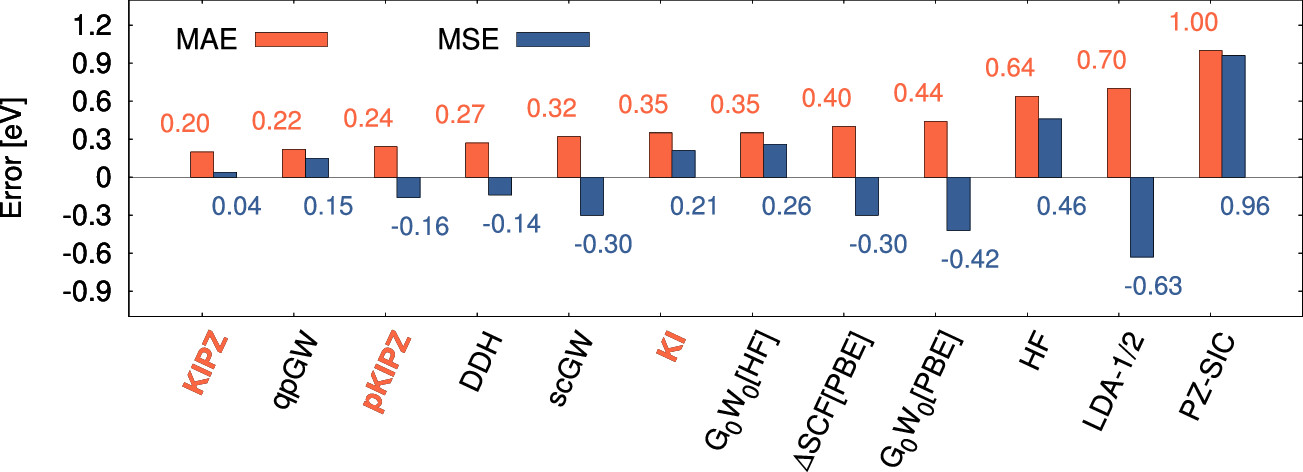
\includegraphics[width=\columnwidth]{figures/colonna_2019_gw100_ip.jpeg}

                        \end{minipage}

                        \hspace{0.5em}

                        \begin{minipage}{0.55\textwidth}
                            \begin{minipage}{0.5\textwidth}
                                    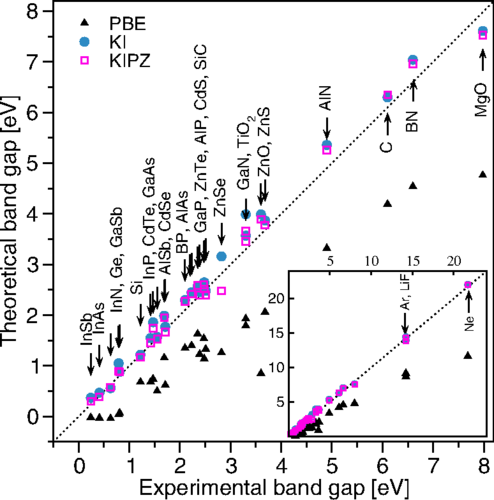
\includegraphics[width=0.9\textwidth,valign=t]{figures/nguyen2018_bandgaps.png}
                            \small
                            \begin{center}
                            \begin{tabular}{c c S[table-format = 2.2] S[table-format = 2.2] S[table-format = 2.2] S[table-format = 2.2] S[table-format = 2.2] S[table-format = 2.2] S[table-format = 2.2] S[table-format = 2.2] S[table-format = 2.2]}
                                                                  &             & {PBE} & {G\textsubscript{0}W\textsubscript{0}} & {KI} & {KIPZ} & {QSG$\tilde{\mathrm{W}}$} \\
                                \midrule
                                \midrule
                                \multirow{2}{*}{$E_\mathrm{gap}$} &
                                {MAE (eV)}                        & 2.54        & 0.56  & 0.27                                   & 0.22 & 0.18                               \\
                                                                  & {MAPE (\%)} & 48.28 & 12.10                                  & 7.09 & 5.37   & 4.46                      \\
                                \midrule
                                \multirow{2}{*}{IP}               &
                                {MAE (eV)}                        & 1.09        & 0.39  & 0.19                                   & 0.21 & 0.49                               \\
                                                                  & {MAPE (\%)} & 15.58 & 5.71                                   & 2.99 & 3.14   & 7.41
                            \end{tabular}
                        \end{center}
                            \end{minipage}
                            \begin{minipage}{0.45\textwidth}
                                    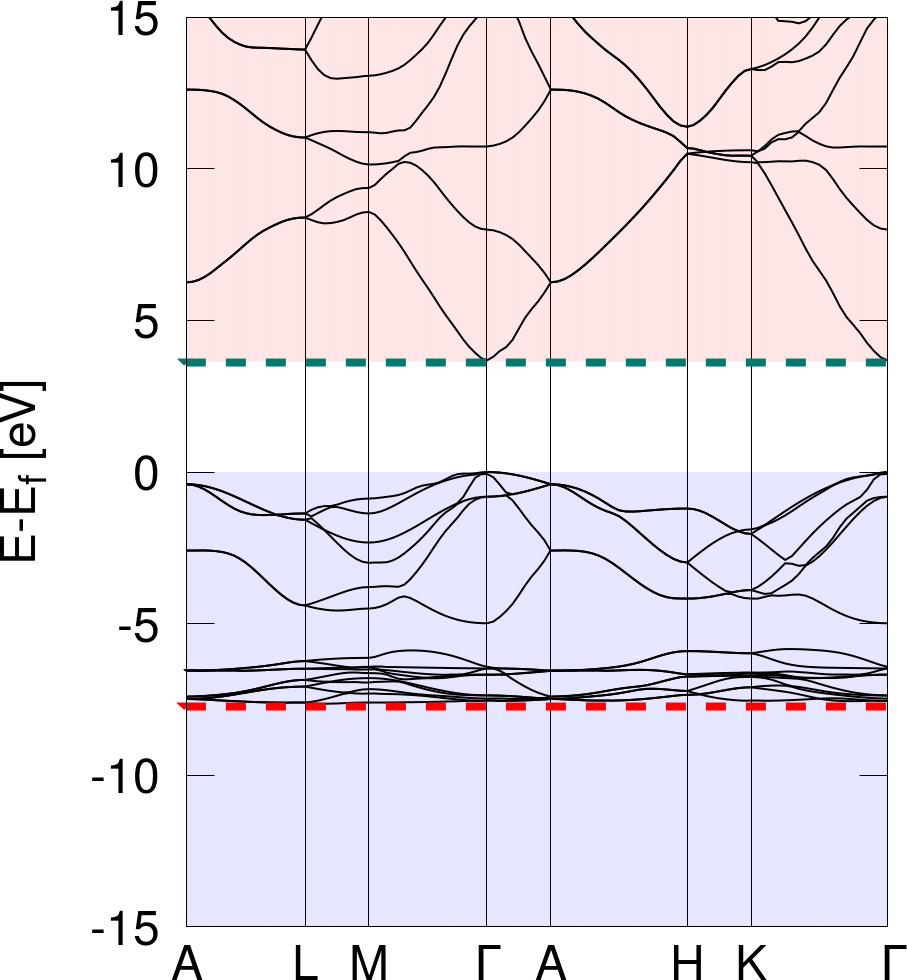
\includegraphics[width=\textwidth,valign=c]{figures/ZnO_ki_trimmed.png}

                                    \vspace{1ex}

                                    The KI band structure of ZnO compared to the experimental band gap and $d$-band position \textcolor{kgrey_light}{\citeauthoryear{Colonna2022}}
                            \end{minipage}
                        \end{minipage}

                    }
                    \hfill

                \end{block}
            \end{column}
        \end{columns}

        \vspace{1.2em}
        \begin{columns}[t]
            \begin{column}{0.47\textwidth}
                \begin{block}{4. What does running \texttt{koopmans} look like?}

                    \hbox{
                        \begin{minipage}[t]{0.44\columnwidth}
                            Koopmans takes a single \texttt{JSON} file as input e.g. for bulk silicon
                            \vspace{0.2em}
                            \inputminted[fontsize=\tiny, autogobble, breaklines]{json}{scripts/si_ki.json}
                        \end{minipage}
                        \hspace{0.025\columnwidth}
                        \begin{minipage}[t]{0.5\columnwidth}
                            Running from the command line looks like this:
                            \vspace{0.3em}
                            \inputminted[fontsize=\tiny, autogobble, breaklines]{shell-session}{scripts/si_ki.out}
                        \end{minipage}
                    }
                    \hfill
                    \vspace{0.86em}

                \end{block}

            \end{column}

            \begin{column}{0.47\textwidth}
                \setbeamercolor{block title}{bg=white, fg=white}
                \begin{block}{\vphantom{P}}
                    \vspace{-2.8ex}
                    or run with \texttt{python}:
                    \inputminted[fontsize=\tiny, autogobble, breaklines]{python}{scripts/si.py}
                \end{block}

                \vspace{1em}
                \setbeamercolor{block title}{bg=kgrey, fg=white}
                \begin{block}{References, affiliations, and acknowledgements}
                    \vspace{0.4em}
                    \hspace{-2em}
                    \begin{minipage}{0.45\textwidth}
                        \AtNextBibliography{\tiny}
                        \printbibliography
                    \end{minipage}
                    \begin{minipage}{0.575\textwidth}
                        \tiny
                        \setbeamercolor{enumerate item}{fg=kgrey}
                        \begin{enumerate}
                            \item Theory and Simulation of Materials (THEOS), \'Ecole Polytechnique F\'ed\'erale de Lausanne, 1015 Lausanne, Switzerland
                            \item National Centre for Computational Design and Discovery of Novel Materials (MARVEL), \'Ecole Polytechnique F\'ed\'erale de Lausanne, 1015 Lausanne, Switzerland
                            \item Laboratory for Neutron Scattering and Imaging, Paul Scherrer Institute, 5232 Villigen, Switzerland
                            \item Laboratory for Materials Simulations, Paul Scherrer Institut, 5232 Villigen, Switzerland
                        \end{enumerate}
                        \vspace{1em}
                        This work was supported by the Swiss National Science Foundation (SNSF) through its National Centre of Competence in Research (NCCR) MARVEL and Grants 179138 and 213082.
                    \end{minipage}

                    \vspace{0.45ex}

                    % \vspace{0.8em}
                    % 
\includegraphics[height=0.07\columnwidth]{/home/elinscott/Pictures/epfl_logos/red_cropped.eps}
                    % \hfill
                    % 
\includegraphics[height=0.07\columnwidth]{figures/psi_trimmed.png}
                    % \hfill
                    % 
\includegraphics[height=0.07\columnwidth]{figures/marvel_trimmed.png}
                    % \hfill
                    % \includegraphics[height=0.07\columnwidth]{/home/elinscott/Pictures/snsf_logos/SNF_logo_standard_print_color_pos_e.eps}
                    % \vspace{0.5em}

                \end{block}
                % \begin{beamercolorbox}[wd=\textwidth,sep=1em]{logos}
                % \end{beamercolorbox}

            \end{column}
        \end{columns}

        \vspace{1.25em}

    \end{beamercolorbox}

    \setbeamercolor{footer}{fg=kgrey,bg=white}
    \begin{beamercolorbox}[wd=\textwidth,sep=1em]{footer}
        \begin{minipage}{0.55\textwidth}
        \includegraphics[width=0.3\columnwidth]{/home/elinscott/Pictures/snsf_logos/SNF_logo_standard_print_color_pos_e.eps}
        \hspace{0.01\columnwidth}
        \tiny The National Centres of Competence in Research (NCCRs) are a funding scheme of the Swiss National Science Foundation
        \end{minipage}
        \hfill
        \begin{minipage}{0.3\textwidth}
            \raggedleft
            \bf \large ... go to {\ttfamily \bf \large koopmans-functionals.org} to find out more!
        \end{minipage}
    \end{beamercolorbox}

\end{frame}
% \setlength{\myimscale}{0.08\textwidth}
% \begin{tikzpicture}[every node/.style={color=kgrey}]
%     \node[inner sep=0pt] (logo) at (3\myimscale,0\myimscale)
%     {
\includegraphics[width=0.7\textwidth]{figures/k_grey_on_transparent.png}};
%     \node[rectangle, draw, thick, minimum width=5.75\myimscale, minimum height=3.5\myimscale, outer sep=0, label=above:linearisation,
%         path picture={
%                 \node at (path picture bounding box.center){
%                     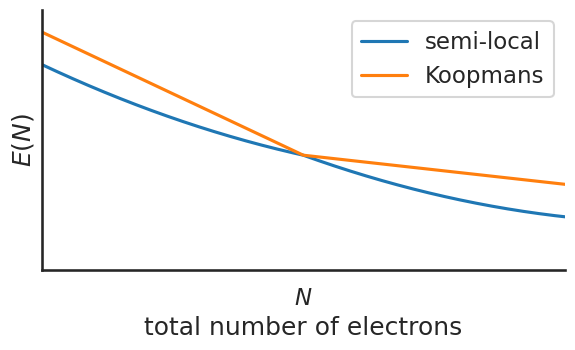
\includegraphics[width=5.75\myimscale]{figures/linearisation.png}
%                 };
%             }] (linear) at (0\myimscale,5.2\myimscale) {};
%     \node[rectangle, draw, thick, minimum width=5.75\myimscale, minimum height=3.5\myimscale, outer sep=0, label=above:screening,
%         path picture={
%                 \node at (path picture bounding box.center){
%                     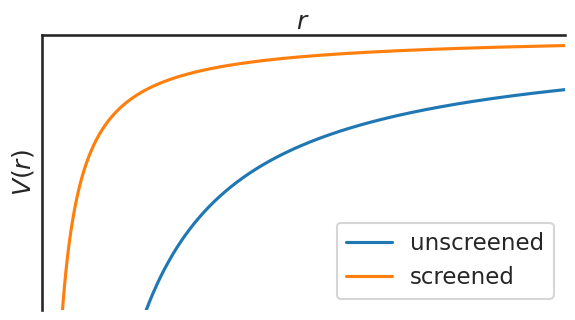
\includegraphics[width=5.75\myimscale]{figures/screening.png}
%                 };
%             }] (screening) at (6.25\myimscale,5.2\myimscale) {};
%     \node[rectangle, minimum width=2.5\myimscale, minimum height=3.5\myimscale, outer sep=0,
%         path picture={
%                 \node at ([yshift=-0.05\myimscale]path picture bounding box.center){
%                     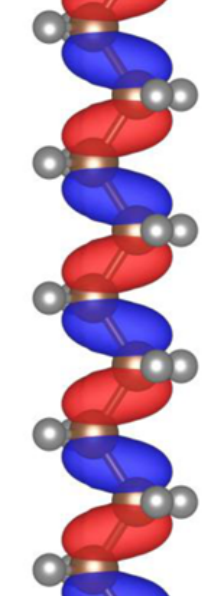
\includegraphics[width=2.5\myimscale]{figures/fig_nguyen_canonical_orbital.png}
%                 };
%             }] (bloch) at (-1.5\myimscale,-5.2\myimscale) {};
%     \node[rectangle, minimum width=2.5\myimscale, minimum height=3.5\myimscale, outer sep=0,
%         path picture={
%                 \node at ([yshift=1.5\myimscale]path picture bounding box.center){
%                     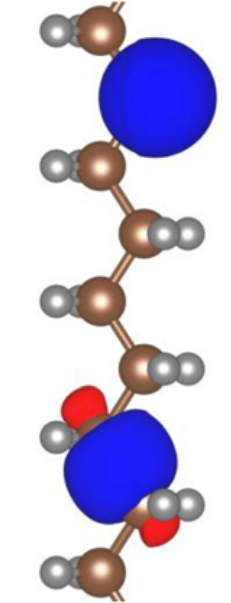
\includegraphics[width=2.6\myimscale]{figures/fig_nguyen_variational_orbital.png}
%                 };
%             }] (wannier) at (1.5\myimscale,-5.2\myimscale) {};
%     \node[rectangle, draw, thick, minimum width=5.75\myimscale, minimum height=3.5\myimscale, outer sep=0, label=below:localisation,
%     ] (localisation) at (0\myimscale,-5.2\myimscale) {};
%     \node[rectangle, draw, thick, minimum width=5.75\myimscale, minimum height=3.5\myimscale, outer sep=0, label=below:automation,
%         path picture={
%                 \node at (path picture bounding box.east){
%                     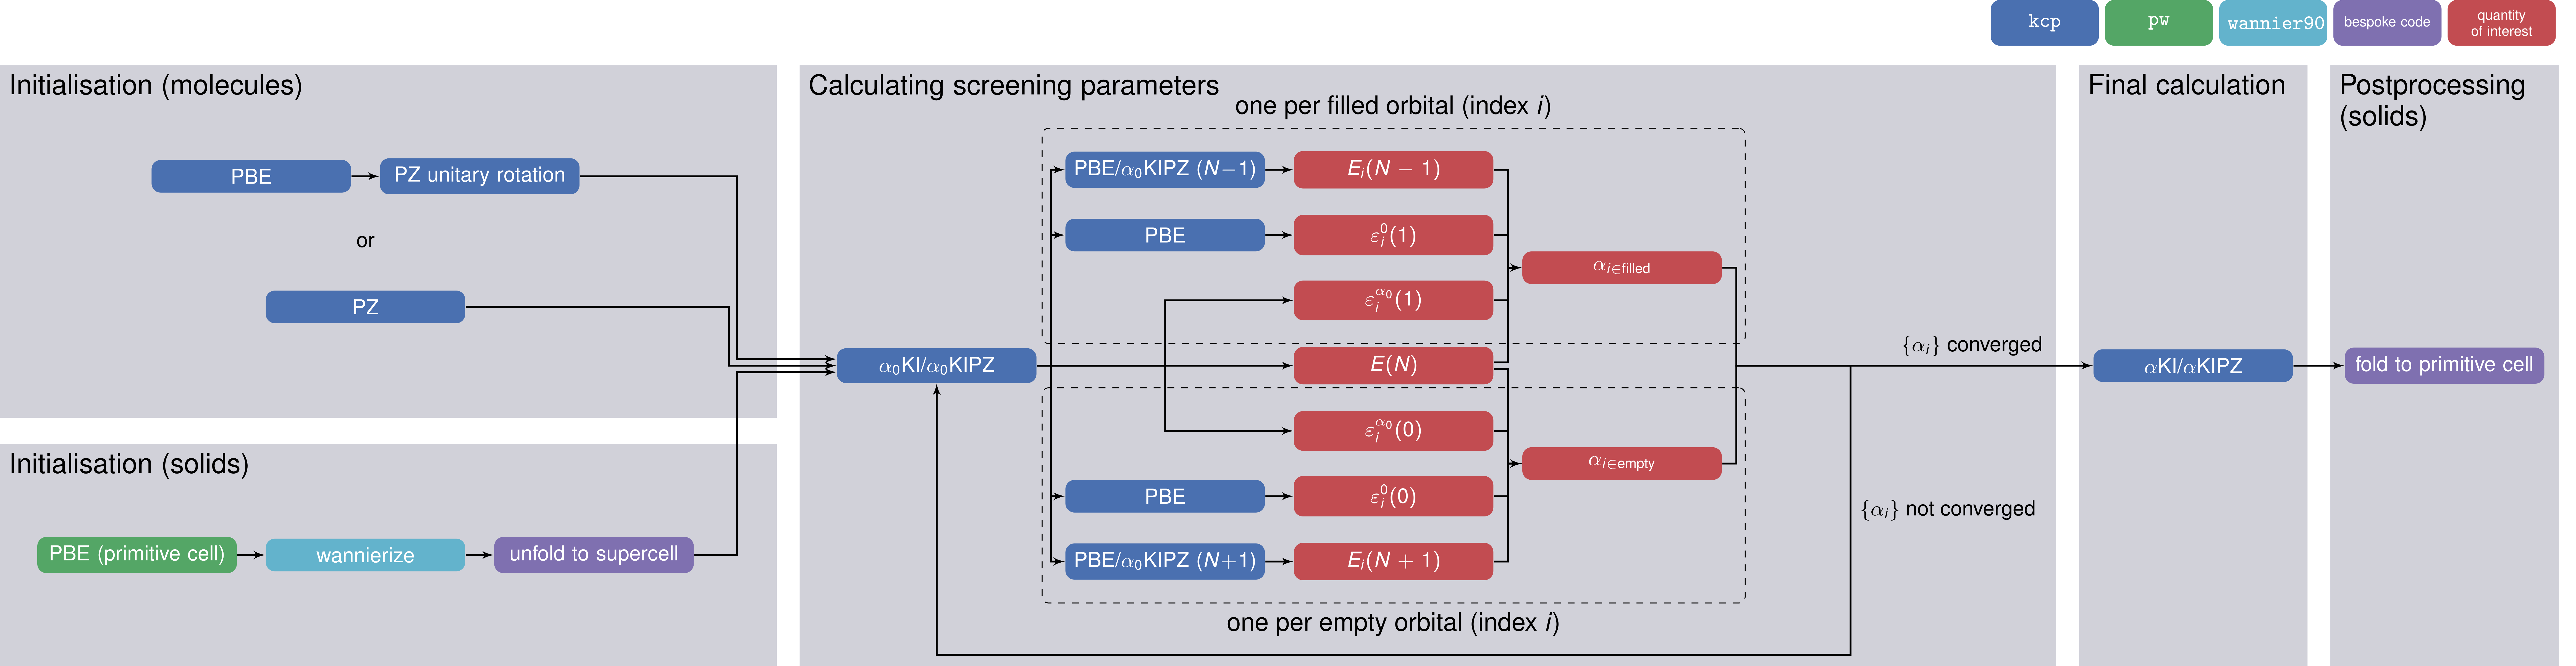
\includegraphics[width=15\myimscale]{figures/dscf_workflow.png}
%                 };
%             }] (workflow) at (6.25\myimscale,-5.2\myimscale) {};
%     \draw[thick, -{Latex[round]}] (bloch) -- (wannier);
% \end{tikzpicture}

\end{document}
